\documentclass[tikz,border=5pt]{standalone}
\usepackage{tikz}
\usetikzlibrary{arrows.meta,3d,decorations.pathreplacing}

% Atlas color palette
\definecolor{AtlasTeal}{HTML}{5BA4A4}
\definecolor{AtlasWarm}{HTML}{C17F59}
\definecolor{AtlasSage}{HTML}{7A9E7E}
\definecolor{AtlasTealLight}{HTML}{D4E8E8}
\definecolor{AtlasWarmLight}{HTML}{F0DED3}

\begin{document}
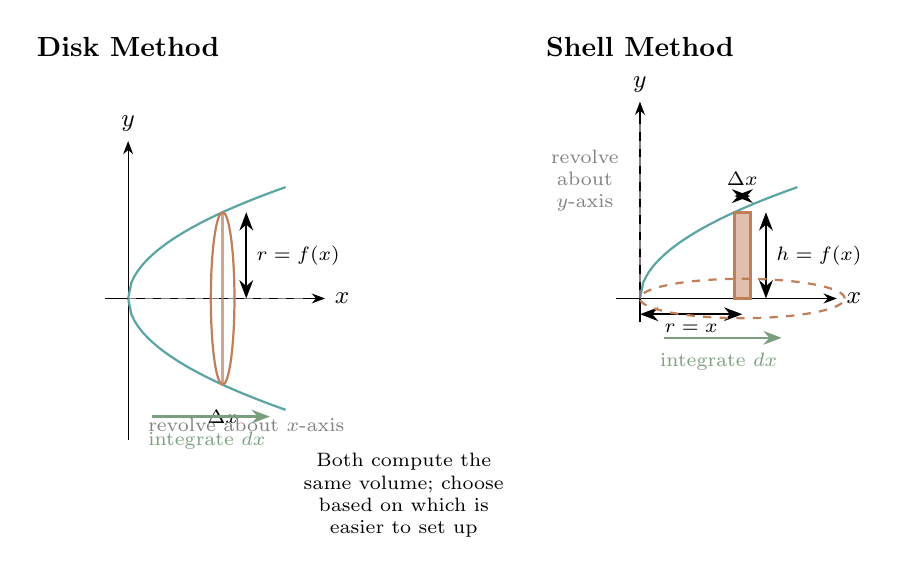
\begin{tikzpicture}[>=Stealth]
    
    % ========== LEFT: DISK METHOD ==========
    \begin{scope}[shift={(-3.5,0)}]
        \node[font=\bfseries] at (0,3.2) {Disk Method};
        
        % Axes
        \draw[->] (-0.3,0) -- (2.5,0) node[right, font=\small] {$x$};
        \draw[->] (0,-1.8) -- (0,2) node[above, font=\small] {$y$};
        
        % Curve y = sqrt(x)
        \draw[AtlasTeal, thick, domain=0:2, samples=50] plot (\x, {sqrt(\x)});
        \draw[AtlasTeal, thick, domain=0:2, samples=50] plot (\x, {-sqrt(\x)});
        
        % A disk slice (vertical)
        \draw[AtlasWarm, very thick, fill=AtlasWarmLight, opacity=0.7] 
            (1.2, -1.095) -- (1.2, 1.095);
        \draw[AtlasWarm, thick] (1.2, 0) ellipse (0.15 and 1.095);
        
        % Disk annotation
        \draw[<->, thick] (1.5, 0) -- node[right, font=\scriptsize] {$r = f(x)$} (1.5, 1.095);
        \node[below, font=\scriptsize] at (1.2, -1.3) {$\Delta x$};
        
        % Axis of revolution indicator
        \draw[dashed, gray] (0, 0) -- (2.3, 0);
        \node[font=\scriptsize, gray] at (1.5, -1.6) {revolve about $x$-axis};
        
        % Integration direction
        \draw[->, thick, AtlasSage] (0.3, -1.5) -- (1.8, -1.5);
        \node[font=\scriptsize, AtlasSage] at (1, -1.8) {integrate $dx$};
    \end{scope}
    
    % ========== RIGHT: SHELL METHOD ==========
    \begin{scope}[shift={(3,0)}]
        \node[font=\bfseries] at (0,3.2) {Shell Method};
        
        % Axes
        \draw[->] (-0.3,0) -- (2.5,0) node[right, font=\small] {$x$};
        \draw[->] (0,-0.3) -- (0,2.5) node[above, font=\small] {$y$};
        
        % Curve y = sqrt(x)
        \draw[AtlasTeal, thick, domain=0:2, samples=50] plot (\x, {sqrt(\x)});
        
        % A shell slice (vertical rectangle)
        \fill[AtlasWarm, opacity=0.5] (1.2, 0) rectangle (1.4, 1.095);
        \draw[AtlasWarm, very thick] (1.2, 0) rectangle (1.4, 1.095);
        
        % Shell annotations
        \draw[<->, thick] (1.6, 0) -- node[right, font=\scriptsize] {$h = f(x)$} (1.6, 1.095);
        \draw[<->, thick] (0, -0.2) -- node[below, font=\scriptsize] {$r = x$} (1.3, -0.2);
        
        % Delta x
        \draw[<->, thick] (1.2, 1.3) -- node[above, font=\scriptsize] {$\Delta x$} (1.4, 1.3);
        
        % Axis of revolution indicator
        \draw[dashed, gray] (0, 0) -- (0, 2.3);
        \node[font=\scriptsize, gray, text width=1.5cm, align=center] at (-0.7, 1.5) {revolve about $y$-axis};
        
        % Integration direction
        \draw[->, thick, AtlasSage] (0.3, -0.5) -- (1.8, -0.5);
        \node[font=\scriptsize, AtlasSage] at (1, -0.8) {integrate $dx$};
        
        % Cylindrical shell suggestion
        \draw[AtlasWarm, thick, dashed] (1.3, 0) ellipse (1.3 and 0.25);
    \end{scope}
    
    % Center comparison note
    \node[font=\scriptsize, text width=3cm, align=center] at (0, -2.5) 
        {Both compute the same volume; choose based on which is easier to set up};

\end{tikzpicture}
\end{document}
